\documentclass[a4paper,12pt]{third-rep}

\newcommand{\uIP}{$\mu{}$IP}
\newcommand{\mm}{\textrm{mm}}
\newcommand{\cm}{\textrm{cm}}
\newcommand{\s}{\textrm{s}}
\newcommand{\ms}{\textrm{ms}}
\newcommand{\Hz}{\textrm{Hz}}
\newcommand{\kHz}{\textrm{kHz}}
\newcommand{\MHz}{\textrm{MHz}}
\newcommand{\KB}{\textrm{KB}}
\newcommand{\dC}{\ensuremath{^\circ\textrm{C}}}

\newenvironment{gcoderegs}%
{\vspace{\itemsep}\hspace{\stretch{1}}}%
{\hspace{\stretch{1}}\vspace{\itemsep}}
\newcommand{\reg}[2]{\textbf{#1:}\hspace{1ex}$#2$\hspace{1.5em}}

%\includeonly{chapter1}

\usepackage{url}
\usepackage{verbatim}
\usepackage{booktabs}

\title{Improving the Makerbot 3D Printer}
\author{Jonathan Heathcote}
\supervisor{Alasdair Rawsthorne}
\reportyear{2012}

%% this defines the file that contains the text of the abstract, there
%% must be one of these by the time you submit your report.
\abstractfile{abstract.tex}

%% this defines the file that contains the acknowledgements (it can be
%% omitted if you don't feel like thanking anyone
\thanksfile{thanks.tex}

% Uncomment the following line if you want to change the name of the
% Bibliography to References
\renewcommand{\bibname}{References}

%%%%%%%%%%%%%%%%%%%%%%%%%%%%%%%%%%%%%%%%%%%%%%%%%%%%%%%%%%%%%%%%%%%%%%%%%%%%%%%%

\begin{document}
	% Front matter
	\dotitleandabstract
	
	\tableofcontents
	\listoffigures
	\listoftables
 
	% Chapters
	\chapter{Introduction}
	
	3D Printing is an additive manufacturing process where computer models of
	objects are reproduced in a physical form. Various technologies exist...
	
	\section{Applications}
	
	\section{Printer Technologies}
	
	\section{Personal 3D Printers}
	
	\section{Makebed}
	
		\subsection{Motivation}
		
		\subsection{Goals}

	\chapter{Background}
	
	\label{sec:background}
	
	In this chapter the background of the project is described. The existing state
	of 3D printer electronics is described followed by an introduction to the
	tasks carried out by the firmware that drives them. Afterwards the ARM based
	`Mbed' microcontroller used in this project is introduced followed by
	`FreeRTOS', the operating system the project is built on.
	
	\section{Printer Electronics}
		
	\section{Firmware}
		
		\subsection{G-code}
		
		\subsection{Mechanical Compensation}
		
		\subsection{Design}
	
	\section{Microcontrollers}
		
		\subsection{ARM}
		
		\subsection{Mbed}
	
	\section{Real-Time Operating Systems}
		
		\subsection{Diferrences From Non-Real-Time Systems}
		
		\subsection{FreeRTOS}
		
			\subsubsection{Tasks}
			
			\subsubsection{Queues \& Mutexes}

	\chapter{Design}
	
	\section{Electronics}
		
		\subsection{Microcontroller}
		
		\subsection{Stepper Control}
		
		\subsection{Heater \& DC Motor Control}
	
	\section{Firmware}
		
		\subsection{FreeRTOS}
		
		\subsection{\uIP}
		
		\subsection{G-Code Interpreter}
		
		\subsection{System Control}
		
		\subsection{Stepper Control}

	\chapter{Implementation}
	
	\label{sec:implementation}
	
	This chapter describes the implementation of the system in detail. First the
	electronics produced are described and followed by an explanation of the
	firmware which drives them. Finally, safety considerations and a brief
	discussion of the development methodology used is presented.
	
	\section{Electronics}
		
		Two circuits were produced, one which hosts the Mbed and the electronics
		needed to drive the heaters, motors and temperature sensors and another
		which provides an interface between the end-stops and stepper controller
		boards.
		
		The main board will host the Mbed, electronics for controlling heaters and
		motors, reading from temperature sensors and connections for the stepper
		controller boards (figure \ref{fig:electronicsDiagram}). A second board is
		used for the end-stop electronics as these parts may be replaced separately
		from the main electronics and connect via the existing stepper controller
		interface. The completed system, as installed in the printer, is shown in
		figure \ref{fig:electronicsPhoto} with the major components labelled.
		
		To keep the system easy to build requiring readily available tools, 0.1"
		spaced electronics were used throughout. These are easy to work with using
		only a standard soldering iron and basic tools. Components of this size can
		also be used for prototyping with a solderless breadboard.
		
		\begin{figure}
			\includegraphics[width=1\textwidth]{diagrams/electronicsDiagram.pdf}
			\caption{Components of the main board}
			\label{fig:electronicsDiagram}
		\end{figure}
		
		\begin{figure}
			\includegraphics[width=1\textwidth]{diagrams/electronicsPhoto.pdf}
			\caption{Electronics installed with key components labelled}
			\label{fig:electronicsPhoto}
		\end{figure}
		
		\subsection{Layout \& Board}
			
			A prototyping board designed for working with DIP (Dual In-line Package)
			components such as the Mbed was selected (Figure \ref{fig:dipBoard}(B)).
			Conventional strip board (\ref{fig:dipBoard}(A)) is not ideal for these
			components as it would require many connections to be cut between the
			columns of pins. 
			
			\begin{figure}
				\includegraphics[width=1\textwidth]{diagrams/dipBoard.pdf}
				\caption{Types of prototyping board}
				\label{fig:dipBoard}
			\end{figure}
			
			\begin{figure}
				\includegraphics[width=1\textwidth]{diagrams/mainBoard.pdf}
				\caption{Top-level layout of main board (reset button and power
				         connections not shown)}
				\label{fig:mainBoard}
			\end{figure}
			
			The main board contains electronics for both low-power systems such as the
			Mbed and high-power systems such as the heater and motors and electrical
			interference between these parts must be minimised. The high and lower
			power parts have been kept physically separate on the board (figure
			\ref{fig:mainBoard}), each with their own power supply connections. The
			board also has a continuous track covering the whole board which can be
			connected to ground (known as a ground plane), helping reduce
			noise \cite{pcb_design_notes}.
			
			A full circuit schematic and pin-out for the board is given in Appendix
			\ref{sec:mainboardDiagrams}.
		
		\subsection{Heaters \& DC Motors}
			
			\label{sec:heatersAndMotors}
			
			The heaters and DC motors in the extruder and platform operate at a higher
			voltage and are considerably higher-current than the microcontroller can
			provide on its output pins. To control these a transistor can be used.
			Transistors act like a switch which allows high-power components to be
			switched on and off using only a small current from the Mbed. An
			IRLU8729PbF MOSFET (Metal Oxide Field Effect Transistor) was selected as
			it can switch large loads up to 58A with very little on-resistance
			(reducing energy wastage through heat) \cite{MOSFET}.
			
			\begin{figure}
				\includegraphics[width=1\textwidth]{diagrams/mosfetDiagram.pdf}
				\caption{Metal Oxide Semiconductor Field Effect Transistor (MOSFET)}
				\label{fig:mosfetDiagram}
			\end{figure}
			
			A MOSFET has three connections called the gate, drain and source
			(Figure \ref{fig:mosfetDiagram}). When the voltage between the gate and
			source is 0V, no current flows from the drain to the source. As the
			voltage between the gate and drain are increased, the current allowed to
			flow increases rapidly when it passes a certain threshold (Figure
			\ref{fig:mosfetPerformance}). By connecting the gate to a pin on the
			Mbed and the source to ground, a large current from a device such as a
			heater or motor attached to the drain can be switched.
			
			\begin{figure}
				\includegraphics[width=1\textwidth]{diagrams/mosfetPerformance.pdf}
				\caption{IRLU8729PbF Typical Transfer Characteristics (reproduced from
				`Fig 3', \cite{MOSFET})}
				\label{fig:mosfetPerformance}
			\end{figure}
			
			The behaviour of a MOSFET when the gate is left floating (disconnected) is
			generally undefined and can damage the component. When the Mbed powers on
			its output pins default to a floating state which could cause a MOSFET to
			unexpectedly switch on or become damaged. To prevent this happening the
			gate is connected to ground via a resistor. When the output pin is
			floating the gate is pulled to 0V by the resistor. When the output of the
			pin is not floating, the gate is pulled to that voltage overriding the
			pull-down resistor. A high resistance value is used so that the Mbed can
			easily override the pull-down resistor. Figure \ref{fig:mosfetUsage} shows
			the circuit used to control the two heaters and two motors using a MOSFET
			and pull-down resistor.
			
			\begin{figure}
				\includegraphics[width=1\textwidth]{diagrams/mosfetUsage.pdf}
				\caption{Example MOSFET circuit with pull-down resistor}
				\label{fig:mosfetUsage}
			\end{figure}
			
			When driving motors, a `flyback diode' is usually used to prevent a
			voltage spike occurring when the power is removed from the motor. This
			voltage spike is caused by the magnetic field in the motor's coils
			collapsing. This is not included in the circuit as the MOSFETs used
			already contain an appropriate diode.
			
			It should be noted that this circuit does not allow the motors to be
			driven in both directions as this is not needed by the printer. If this
			was required, a more complex circuit (such as an H bridge) would be
			needed.
		
		\subsection{Thermistors}
			
			\label{sec:thermistor}
			
			To measure the temperature of the heaters, thermistors are used. The
			resistance of a thermistor changes non-linearly with temperature and can
			be modelled using an equation derived from the Steinhart-Hart
			Equation \cite{Steinhart1968497}:
			\begin{equation}
				\frac{1}{T} = \frac{1}{T_0} + \frac{1}{\beta} \ln \left( \frac{R}{R_0} \right)
				\label{equ:steinhart}
			\end{equation}
			Where $T$ and $R$ are the current temperature and resistance of the
			thermistor, $T_0$ and $R_0$ are the temperature and resistance at a
			reference temperature and $\beta$ is a characteristic constant for the
			device available in the data-sheet.
			
			Using the Analog-to-Digital converter in the Mbed, voltages, but not
			resistances, can be read directly. As a result, a potential divider
			(figure \ref{fig:potentialDiv}) is used to produce a measurable voltage
			which is proportional to the resistance to measure it indirectly.
			\begin{figure}
				\includegraphics[width=1\textwidth]{diagrams/potentialDiv.pdf}
				\caption{Potential divider}
				\label{fig:potentialDiv}
			\end{figure}
			A reference voltage $V_\textrm{ref}$ is placed across two resistors,
			$R_1$ and $R_2$, and the voltage between them at $V$ is measured. The
			relationship between these variables is
			\begin{equation}
				V = V_\textrm{ref} \frac{R_2}{R_1 + R_2}
			\end{equation}
			Thus, if the thermistor is placed as $R_2$, the resistance can be
			calculated using
			\begin{equation}
				R_2 = V_\textrm{ref} \frac{R_1}{V - V_\textrm{ref}}
				\label{equ:potdiv}
			\end{equation}
			
			The value of $R_1$ was chosen to evenly spread the voltages from the
			expected range of thermistor resistances over the full range of 0 to
			$V_\textrm{ref}$ volts. This maximises the utilisation of the analog to
			digital converter available over the temperature ranges used.
			
			Using (\ref{equ:steinhart}) and (\ref{equ:potdiv}) with a potential
			divider circuit will allow the temperature of the thermistor to be
			measured.
			
		
		\subsection{Stepper Motors}
			
			The stepper controllers chosen accept TTL signals and connect via a
			ten-pin insulation displacement connector (IDC). An IDC socket was
			placed on the board and the pins connected directly to the Mbed and
			ground plane as required.
		
		\subsection{End-stops}
			
			Optical end-stops consist of a photo-interrupter containing an infra-red
			LED and a photo-transistor arranged across a gap (Figure
			\ref{fig:endstop}). Photons from the LED activate the photo-transistor
			allowing current to flow but, when the gap is blocked, the transistor is
			switched off and no current flows.
			
			\begin{figure}
				\includegraphics[width=1\textwidth]{diagrams/endstop.pdf}
				\caption{Photo-interrupter with a photo-transistor in a Darlington pair}
				\label{fig:endstop}
			\end{figure}
			
			Due to problems sourcing the interface boards for the end-stops, a circuit
			was built which is compatible with the stepper-controller interface. $+5V$
			and ground are provided and a TTL logic signal is expected by the
			interface. To ease debugging, an indicator LED was also added which is lit
			when the end-stop is unobstructed.
			
			The LED in the photo-interrupter is driven via a current-limiting
			resistor and the signal output and indicator LED are connected through
			the photo-transistor. A pull-down resistor is used to pull the signal
			to ground when the photo-transistor is powered off.
			
			The circuitry is placed on a board with cables running to each end-stop
			(shown mounted in figure \ref{fig:endstopInstalled}) and to each of the
			CAT-5 sockets on the stepper controller boards. Strain-relief is included
			so that the connections are not damaged if the cables are caught in the
			machine. A circuit diagram is provided in appendix
			\ref{sec:endstopDiagram}.
			
			\begin{figure}
				\includegraphics[width=1\textwidth]{diagrams/endstopInstalled.pdf}
				\caption{Photo-interrupter endstop being interrupted by the X-axis}
				\label{fig:endstopInstalled}
			\end{figure}
			
		\subsection{Power}
			
			The printer uses an ATX power supply unit (PSU) commonly found in desktop
			computers. A 20-pin connector containing both power and various control
			signals for the power supply (see table \ref{tab:atxConnectors}) is used
			to power the main board.
			
			\begin{table}[here]
				\centering
				\begin{tabular}{l l l}
					\toprule
					Signal & Colour & Notes\\
					\midrule
					Ground & Black  & \\
					+3.3V  & Orange & $\pm5\%$  Tolerance (Unused) \\
					+5V    & Red    & $\pm5\%$  Tolerance \\
					+12V   & Yellow & $\pm5\%$  Tolerance \\
					-12V   & Blue   & $\pm10\%$ Tolerance (Unused) \\
					\addlinespace
					Power Good  & Gray   & Signal asserted when all voltages are correct
					                       and stable \\
					+5V Standby & Purple & Power available at all times (Max 2A) \\
					+3.3V Sense & Brown  & Unused \\
					Power On    & Green  & Active-Low signal pulled up to +5V \\
					
					\bottomrule
				\end{tabular}
				
				\caption{20-pin ATX Connector Signals\cite{ATX}}
				\label{tab:atxConnectors}
			\end{table}
			
			The Mbed is connected to the 5V standby supply allowing it to remain
			connected to the network and power on the system on demand. The maximum
			power consumption of the Mbed is 200mA, well within the ratings of the ATX
			specification \cite{mbed}. The Mbed's on-board regulator provides a
			regulated 3.3V supply used by the Mbed and the low-power electronics
			attached to it. The 3.3V supply from the PSU is not used because the
			regulator in the Mbed offers a cleaner supply which is always available.
			
			To allow the PSU to be turned on by the Mbed, the power on signal is
			attached to a GPIO pin.  Because the Mbed is a 3.3V logic device a MOSFET
			is used to connect the 5V Power On signal to ground (thus turning on the
			Power Supply) using the 3.3V signal from the Mbed.
		
		\subsection{Ethernet}
			
			Ethernet requires relatively complex circuitry to drive it. With the
			exception of the Ethernet magnetics, this is provided on-board the Mbed. A
			jack containing the magnetics (figure \ref{fig:jackMagnetics}) was used to
			complete the system.
			
			\begin{figure}
				\includegraphics[width=1\textwidth]{diagrams/jackMagnetics.pdf}
				\caption{X-ray of RJ45 sockets with and without integrated magnetics
				         \cite{raspimag}}
				\label{fig:jackMagnetics}
			\end{figure}
	
	\section{Firmware}
		
		In this section the firmware for the Mbed is described, starting with the
		infrastructure required for development on FreeRTOS on the Mbed and then
		moving on to the major components of the system. Finally the safety
		precautions taken and the tools and development practices used are outlined.
		
		\subsection{FreeRTOS on the Mbed}
			
			\label{sec:compiler}
			
			The Mbed is designed for use with a web-based IDE and compiler
			\cite{mbedcompiler}. This system is not appropriate for use in the project
			as the process of uploading code to be compiled is laborious and the
			compilation options restricted.
			
			The CodeSourcery G++ None-EABI toolchain includes a GCC ARM cross-compiler,
			linker and LibC compiled for various ARM based microcontrollers. It was
			selected over closed-source alternatives because it has a large community of
			users and produces reasonable code.
			
			An unofficial port of FreeRTOS for the Mbed is available designed for the
			CodeSourcery toolchain. It provides a base FreeRTOS configuration with a
			demonstration \uIP{} based web server as well as other simple operating
			system demos. Also included are headers for the ARM Cortex Microcontroller
			Software Interface Standard (CMSIS) which defines a common interface for
			ARM Cortex microcontrollers \cite{cmsis}. Finally, headers defining macros
			and pointers for all control registers in the Mbed are included.
			
			Appendix \ref{sec:compilation} contains specific compilation instructions
			for the final system with the CodeSourcery toolchain.
		
		\subsection{Temperature Control}
			
			To drive the two heaters an active-feedback loop is used where input from
			a thermistor is used to drive a heater via a MOSFET. The following
			subsections describe how analog values are read by the Mbed and the theory
			and operation of the feedback loop that controls the heaters.
			
			\subsubsection{Analog Input}
				
				The Mbed includes a 12-bit successive-approximation analog-to-digital
				converter (ADC) for reading analog values \cite{lpc1768}. The ADC uses a
				digital-to-analog converter and a comparator to binary search for an
				approximation to the analog value while the input is held constant
				(figure \ref{fig:adc}). Once an appropriate
				number of iterations of the binary search have been carried out, the
				value in the register is returned \cite{maximadc}.
				
				\begin{figure}
					\includegraphics[width=1\textwidth]{diagrams/adc.pdf}
					\caption{Successive-approximation analog-to-digital converter}
					\label{fig:adc}
				\end{figure}
				
				The ADC sampling process takes at least $5\mu{}s$ or approximately 500
				CPU cycles therefore the CPU can carry out another task while the ADC
				process takes place \cite{lpc1768}. Though an interrupt is provided when
				the ADC completes (as well as a direct memory access (DMA) facility),
				this was not used. Instead, a slow-poll is used where the task reading
				from the ADC is suspended for a time typically adequate for ADC
				operation. The temperature sensors are sampled at an extremely low rate
				(around 2Hz) and latency is not important as changes occur very slowly.
				This system is very simple to implement with negligible overhead.
			
			\subsubsection{Heater Control Loop}
				
				A na\"{i}ve controller could simply turn on the heaters whenever the
				temperature drops below some target temperature or `set point' and then
				off when it was met or exceeded. This type of controller can cause the
				temperature to overshoot and fall below the set point as the heating and
				cooling of the system is not immediate. Instead a
				proportional-integral-derivative (PID) controller is used which can
				control heaters which takes into account such behaviours. PID
				controllers are widely used where a process which is not completely
				understood must be controlled \cite{controleng}.
				
				\begin{figure}
					\includegraphics[width=1\textwidth]{diagrams/pid.pdf}
					\caption{PID heater controller schematic}
					\label{fig:pid}
				\end{figure}
				
				Figure \ref{fig:pid} shows a schematic of the PID controller used in the
				system. At time $t$ the comparator calculates the error, $e(t)$, between
				the actual temperature and the set point. A value is calculated from
				this error using a factor proportional to the error, the error
				accumulated over time (integral) and the error's rate of change
				(derivative). These factors are weighted by the constants $K_p$, $K_i$
				and $K_d$ respectively and the result used to control the heater. The
				three weights must be chosen manually to produce sensible behaviour.
				\S\ref{sec:pidtraning} discusses how these values were selected.
				
				The value calculated could be used to control an analog output or
				PWM\footnote{Pulse width modulation (PWM) is a method of approximating
				analog outputs by rapidly switching a signal on and off with a varying
				duty-cycle. This is cheap to implement in hardware and avoids
				inefficiencies in MOSFETs when only partially driven.} or a threshold
				value used to decide whether a heater is on or off (`bang-bang'
				control). Bang-bang control was used as the previous electronics proved
				this method to be adequate.
				
				The PID control loop is executed in its own task twice a second when
				each temperature is read and the heaters switched on and off as
				appropriate. Executing the loop more frequently would not be useful
				because of the slow rate of change in the system. Doing so would also be
				costly due to floating point calculations being carried out in software.
		
		\subsection{Stepper Control}
			
			To drive the stepper controllers, accurately timed pulses must be produced
			to cause the stepper motors to move at the correct speed. These pulses
			also need to be coherent between motors so that the three axes can move
			simultaneously to plot straight paths.
			
			\subsubsection{Principle of Operation}
			
			Before each movement begins, a periodic timer is set based on the
			frequency at which steps must occur and is used to toggle the step signal.
			This is used instead of Bresenham's line algorithm to simplify
			implementation \cite{bresenham}.  Since expensive floating point
			calculations are required for value conversion into machine units, the
			additional calculation introduced is not significant. During each timer
			tick only cheap integer operations are required.
			
			\subsubsection{Timing Constraints}
				
				The stepper controller boards are based on an Allegro A3982 stepper
				controller which defines additional timing requirements. Table
				\ref{tab:stepperTiming} gives the timing constraints for these signals.
				Figure \ref{fig:stepperWave} shows an example waveform with three
				forward steps followed by four backward steps. On the positive edge of
				the step signal the direction is sampled and the motor is stepped.
				
				\begin{figure}
					\includegraphics[width=1\textwidth]{diagrams/stepperWave.pdf}
					\caption{Stepper control signal wave diagram}
					\label{fig:stepperWave}
				\end{figure}
				
				\begin{table}
					\centering
					\begin{tabular}{l l l}
						\toprule
						Period & Meaning & Timing Constraint\\
						\midrule
						$t_{sh}$ & Step high  & $\ge 1\mu{}s$ \cite{allegro} \\
						$t_{sl}$ & Step low   & $\ge 1\mu{}s$ \cite{allegro} \\
						\addlinespace
						$t_{s}$  & Setup time & $\ge 200ns$   \cite{allegro} \\
						$t_{h}$  & Hold time  & $\ge 200ns$   \cite{allegro} \\
						\addlinespace
						$t_{t}$  & Step time  & $\ge 757\mu{}s$ (Experimentally determined) \\
						\bottomrule
					\end{tabular}
					
					\caption{Stepper timing constraints}
					\label{tab:stepperTiming}
				\end{table}
				
				The motors in the printer add an additional timing constraint, $t_t$,
				due the limit on how often they can step defined by the mechanical
				properties of the printer. This is important because the faster the
				stepper is driven, the less torque is available and so the stepper may
				miss steps and fail to move.
			
			\subsubsection{Timer Requirements}
				
				If a stepper is set to run at its maximum speed, steps will be $757\us$
				apart meaning that the signal must be toggled every $379\us$.  Therefore
				the output signals may change at up to $1.32\kHz$.
				
				FreeRTOS provides timing guarantees for scheduling arbitrary delays
				within tasks. Unfortunately, this uses the system timer which ticks at
				$1\kHz$ which is too far low for the frequencies such as those discussed
				above. 
				
				According to the Nyquist-Shannon sampling theorem a frequency of $f\Hz$
				can only be generated by a timer running at $> 2f\Hz$. This means the
				timer resolution must be above $2 \times 1.32\kHz = 2.64\kHz$
				\cite{shannon}. Figure \ref{fig:nyquist} shows `aliasing' caused by
				trying to reproduce a signal at $\frac{2}{3}$ ($> \frac{1}{2}$) the
				frequency of the timer where whole cycles are missing in the output.
				
				\begin{figure}
					\includegraphics[width=1\textwidth]{diagrams/nyquist.pdf}
					\caption{Nyquist-Shannon sampling theorem example with high-frequency
					signal}
					\label{fig:nyquist}
				\end{figure}
				
				The effect of sampling artefacts can cause further inaccuracies. Figure
				\ref{fig:artefacts} shows a signal below $\frac{1}{2}$ of the sampling
				frequency displaying such artefacts. In the worst case when sampling at
				$f\Hz$, a signal change may be $\frac{1}{f}\s$ late. Therefore,
				increasing the sampling frequency decreases the error introduced by such
				artefacts.
				
				\begin{figure}
					\includegraphics[width=1\textwidth]{diagrams/artefacts.pdf}
					\caption{Example of sampling artefacts}
					\label{fig:artefacts}
				\end{figure}
				
				High print quality depends on smooth, even steps, as a result, the timer
				resolution must be not only above $2.64\kHz$ due to the Nyquist-Shannon
				sampling theorem but also be high enough to reduce sampling artefacts to
				an acceptable level. If errors due to artefacts are to be reduced in the
				worst case to, for example, one-hundredth of the step period then a
				frequency of $264\kHz$ is needed.
				
				Increasing the speed of the system timer to such a frequency would make
				the overhead of the scheduler unacceptable and so the FreeRTOS timer
				cannot be used. Instead a hardware timer which interrupts the
				microcontroller causing a light weight interrupt service routine (ISR)
				to run will be needed.
				
				Because the Mbed only provides a limited number of hardware timers, just
				one is used to control all three steppers. As each stepper may not be in
				phase, the time between signals being produced for each stepper can
				become very small, even when the step period is large. This is another
				example of a sampling artefact where the resulting errors are at worst
				$\frac{1}{f}\s$ for a timer running at $f\Hz$. Because the timer is
				already sufficiently fast to make such errors insignificant, no extra
				precision is required when sharing a timer.
				
				The timers provided on board the Mbed consist of a register comparator
				and counter which is incremented by the system clock after being passed
				through a clock divider (figure \ref{fig:timerArch}). The timer was
				configured such that when the counter matches the value in the register,
				the counter is reset and the CPU is interrupted. The timer was
				configured to run at $1\MHz$ which exceeds the $264\kHz$ requirement
				calculated above with some additional margin.
				
				\begin{figure}
					\includegraphics[width=1\textwidth]{diagrams/timerArch.pdf}
					\caption{Mbed timer architecture}
					\label{fig:timerArch}
				\end{figure}
				
				The ISR for the timer interrupt determines for each stepper, whether its
				step signal should be toggled and calculates how long until another
				interrupt is required. The timer compare register is updated, the ISR
				returns and normal program execution resumes.
				
				GCC generates approximately 100 instructions for the ISR taking an
				estimated 250 cycles to execute\footnote{Estimate based on informal
				analysis of the generated assembly code}. Assuming the CPU executes one
				instruction per cycle at $100\MHz$ the amount of CPU time used by the
				ISR in the worst case can be calculated as follows:
				\begin{equation}
					\textrm{Overhead} =
					\frac{\textrm{Interrupts Per Seccond} \times \textrm{ISR Cycles}}
					     {\textrm{Cycles Per Seccond}} =
					\frac{(1.32\times10^3) \times 250}
					     {100\times10^6} = 0.33\%
				\end{equation}
				
				This design results in very little overhead in the system but provides
				very accurately signals to the stepper motors.
			
			\subsubsection{Usage}
				
				An API is provided which allows a number of steps in a given direction
				with a specified period to be sent to a stepper motor. To allow
				sequences of coherent movements to be made, a method which blocks until
				all steps have been completed is also provided. This method uses a
				semaphore which is released by the ISR when all steps have been
				completed. This is also used to temporarily give a higher priority to
				the controlling task during which time the next sequence of steps
				can be started immediately.
		
		\subsection{G-Code Interpreter}
			
			In this subsection there is a discussion of the selection of G-code
			features implemented by the system. Following this, the implementation of
			the parser and interpreter is described.
			
			\subsubsection{Feature Subset Selection}
				
				G-code interpreters support a large variety of features ranging from
				comments and instructions which return data to error checking. As well
				as various language features, the actions available and their precise
				behaviours differ.
				
				To keep the system as simple (and fast) as possible, only features and
				actions required to support the output of Skeinforge's G-code generator
				were implemented.  The resulting language simply supports comments and
				writing to registers.  The syntax supported is given in Backus-Naur Form
				(BNF) in appendix \ref{sec:gcodebnf}.
				
				Actions (and their treatment of registers) were also selected based on the
				output of Skeinforge and include:
				\begin{itemize}
					\item Unit selection
					\item Calibration
					\item Movement
					\item Motor control
					\item Power control
					\item Temperature control
					\item Delays
				\end{itemize}
				A complete description of the actions supported is given in appendix
				\ref{sec:gcodeactions}.
			
			\subsubsection{Parsing}
				
				The G-code subset supported is very simple and so a small parser was
				implemented by hand rather than using a standard parser generator such
				as GNU Bison. Such tools also generate code that is not optimised for
				running on a microcontroller in a real-time environment and would have
				been time consuming to learn.
				
				A simple state machine was built which parses and executes the G-code
				setting and reading registers as described in \S\ref{ref:gcodemachine}.
				When unexpected characters or register values are encountered a flag is
				set and the parser continues from the next character or instruction.
				
				Once each instruction is parsed and the register values set, the values
				are converted into machine units. For example, movements are converted
				into relative movements measured in stepper motor steps and speeds
				converted into step periods measured in timer ticks. These low-level
				commands are then added to the command buffer to be executed by the
				printer controller.
		
		\subsection{Printer Controller}
			
			The printer controller uses a FreeRTOS queue in a high priority task to
			buffer low-level commands from the G-code interpreter. The controller
			consists of a simple loop which executes each command requiring minimal
			processing. As a result, this task spends most of its time blocked waiting
			for actions to complete but responds quickly when required.
		
		\subsection{Network Interface}
			
			The network interface consists of two services built on the \uIP{} stack:
			a G-code transmission interface and a status monitoring interface. \uIP{}
			provides a simple API for sending and receiving data over TCP and UDP
			within applications built within its protosocket and protothread
			frameworks \cite{uIP}.
			
			Protothreads are extremely lightweight threads using cooperative
			multitasking implemented in pure C. These threads do not preserve
			registers or variables during blocking phases of execution and use minimal
			system resources. Protosockets are a simplified UNIX-style socket
			interface built on protothreads. These libraries are designed with
			extremely low-power microcontrollers in mind.  As a result, only a minimal
			application is implemented within the \uIP{} framework which passes data
			from the network immediately to the other parts of the system.
			
			The G-code was initially implemented using TCP but a bug in \uIP{}'s flow
			control implementation meant an alternative implementation was required
			and built on UDP. The two protocols are outlined below along with an
			additional TCP interface used for reporting the system's status.
			
				\subsubsection{TCP G-code Interface}
					
					The TCP G-code interface consists of an open port listening for
					connections. Once connected a client simply sends the G-code to the
					printer and disconnects when finished. Telnet or net-cat (\verb|nc|)
					can be used to send G-code files to the printer, for example
					\begin{verbatim}
						nc 192.168.3.100 1818 -q 0 < model.gcode
					\end{verbatim}
					Where \verb|model.gcode| is the file to send and \verb|193.168.3.100|
					is the IP of the printer.
					
					As the G-code subset supported does not support return values, nothing
					is returned by the printer.
				
				\subsubsection{UDP G-code Interface}
					
					\label{sec:udpimpl}
					
					Unfortunately, as discussed in \S\ref{sec:tcpProblem}, the TCP
					implementation in \uIP{} is incorrect. Due to time constraints this
					was not fixed during the project. Instead a UDP based protocol was
					implemented.
					
					UDP provides a facility for sending datagrams containing a small
					amount of data to a remote host. These datagrams are not guaranteed to
					arrive or to arrive in the order they are sent. They do include a
					checksum and so if a datagram arrives it can be safely be assumed to
					be intact. Finally no flow-control mechanism is provided (excess
					packets are silently dropped). They are, however, lightweight and a
					good base for building custom protocols.
					
					UDP alone cannot be used to send data to the printer and simple
					protocol has been built on top which provides a communications
					channel which is
					\begin{itemize}
						\item Reliable
						\item Unidirectional
						\item Order-guaranteed
						\item Flow-controlled
					\end{itemize}
					
					Figure \ref{fig:datagram} shows the format of datagrams sent between
					the printer and sender. Datagrams are sent to the printer which
					contain a sequence number and a payload whose length can be calculated
					based on the datagram's size (contained in the UDP header). The sender
					then waits for a response from the printer containing the same
					sequence number and a window size. The printer will only respond if a
					datagram with an appropriate sequence number is received discarding
					out-of-order datagrams. If a response with a matching sequence number
					is not received by the sender within a short timeout, the datagram is
					retransmitted. This mechanism facilitates reliable, in-order
					transmission.
					
					The window size returned by the printer is used for flow control and
					is the amount of space in the G-code buffer or the maximum datagram
					size (whichever is smallest). The sender may send up to this amount of
					data to the printer in its next datagram ensuring the printer is
					always sent as much data is it can deal with. If the G-code buffer
					becomes full then the window size will become zero the sender must
					poll the printer until the window size becomes non-zero.
					
					\begin{figure}
						\includegraphics[width=1\textwidth]{diagrams/datagram.pdf}
						\caption{UDP G-code Sender Datagram Format}
						\label{fig:datagram}
					\end{figure}
					
					\S\ref{sec:udpPerformance} discusses the performance and practical
					implications of this protocol and the full specification is given in
					Appendix \ref{sec:udpSpec}.
			
			\subsubsection{Status Interface}
				
				\label{sec:statusInterface}
				
				A simple Telnet-compatible TCP interface (listening on port 2777) was
				implemented that can be used to request the contents of various status
				and debugging variables. As flow control was not necessary, the TCP
				implementation in \uIP{} is adequate for this purpose.
				
				The interface listens for keywords separated by white space and responds
				with tab separated data compatible with GNU Plot. For example:
				\begin{verbatim}
					tmp
					22523	22500	0	11800	12000	1
				\end{verbatim}
				The command \verb|tmp| requests current temperature information. The
				response contains the current temperature, set point (target) and
				whether the heater is on or off for the extruder and the platform.
				Temperature readings are given in degrees Celsius multiplied by 100. This is
				due to the version of LibC provided with the CodeSourcery tool chain not
				supporting printing of floating point values.
				
				A utilities for using the status monitoring facility are described in
				the next section and full documentation for the protocol is given in
				Appendix \ref{sec:statusSpec}.
	
	
	\section{Utilities}
		
		Two utilities for interacting with the printer were written in Python. The
		first, a client implementing the UDP G-code transmission protocol and, the
		second, a utility for conveniently monitoring the printer status. These
		utilities are part of the \verb|makebed.py| command.
		
		For example, the following command will stream the G-code contained in
		\verb|cube.gcode| to the printer:
		\begin{verbatim}
			makebed.py send cube.gcode
		\end{verbatim}
		
		While print jobs are running the status information can be requested or
		polled. For example:
		\begin{verbatim}
			makebed.py get temperature
		\end{verbatim}
		
		Additionally, a simple wrapper, \verb|makebed_live.sh|, is provided written
		in Bash using GNU Plot to plot various pieces of printer status information
		in real-time (figure \ref{fig:makebedlive}).
		
		\begin{figure}
			\includegraphics[width=1\textwidth]{diagrams/makebedlive.pdf}
			\caption{\texttt{makebed live.sh} screen shot}
			\label{fig:makebedlive}
		\end{figure}
		
		Usage information for the utilities can be found in Appendix
		\ref{sec:utilDoc}.
	
	\section{Safety}
		
		Because the system contains heaters and moving parts, safety was a major
		consideration when implementing the system. This section outlines the key
		features used to ensure operation is as safe as possible including
		human-interaction features and fail-safe design.
		
		\subsection{Heater Indicator LEDs}
			
			The two heaters each use an indicator LED on the microcontroller to
			indicate when the heaters are powered on. This enables an operator to
			easily and safely check the state of the heaters during operation.
		
		\subsection{Power-on Behaviour}
			
			On power-on, the PSU is not turned on and so the heaters and motors do not
			receive power. The only way to start the heaters is to open a new
			connection to the printer and send the required PSU and heater
			instructions. This design means that if the printer is powered on
			unintentionally it will not do anything unsafe. It also means that
			resetting the printer has the effect of putting it into a safe state where
			an explicit action is required to restart it.
		
		\subsection{Stop Button}
			
			The electronics connect the Mbed's reset pin to a larger and easier to
			press red button (figure \ref{fig:stop}). Because of the safe power-on
			behaviour and indifference to software failures this button can always but
			the system into a safe state.
			
			\begin{figure}
				\includegraphics[width=1\textwidth]{diagrams/stop.pdf}
				\caption{Emergency stop/reset button}
				\label{fig:stop}
			\end{figure}
		
		\subsection{Watchdog Timer}
			
			The most safety critical software process is that of the heater
			controller. If this routine fails for any reason the heaters may become
			stuck powered on. As over-heating is not as obvious to the operator as for
			example, a jammed axis, this is a particularly dangerous fault.
			
			To catch such faults the Mbed includes a hardware watchdog timer (WDT).
			The WDT contains timer which, upon timing out, resets the system. The WDT
			must be `fed' (reset) periodically to prevent it resetting the system. To
			feed the WDT specific values must be loaded in the correct order into a
			control register. This mechanism can catch bugs which cause the routine to
			jump to a random location, block for an excessive period or otherwise
			become corrupted.
			
			The heater controller loop executes at 2Hz and the WDT is fed at the end
			of each iteration of the control loop. The WDT is set with a timeout of
			two seconds meaning that it should never come close to a timeout except in
			the event of a control loop has failure or the system resources have
			somehow become saturated.
			
			After the WDT has reset the system it enters a safe state where the
			heaters do not have power and are allowed to cool safely.
	
	\section{Methodology \& Tools}
		
		In this section the methodologies used for the implementation of the system
		are discussed followed by the choice of languages and development tools and
		why they were selected. Finally the methods used to debug the firmware
		running on the Mbed are described.
		
		\subsection{Methodology}
		
			Development followed an iterative, bottom-up process where components were
			built, tested and then integrated into the system as a whole.
			
			Prototyping was used heavily in the development of the electronics. The
			major parts of the circuit were initially prototyped on a solderless
			breadboard and powered by a bench power supply (figure
			\ref{fig:breadboard}). In these prototypes, different components could
			easily be swapped in and out of the design and measurements easily taken
			with the system running at different voltages.
			
			\begin{figure}
				\includegraphics[width=1\textwidth]{diagrams/breadboard.pdf}
				\caption{Breadboard with a prototype end-stop circuit}
				\label{fig:breadboard}
			\end{figure}
			
			The UDP protocol was also initially prototyped using a high level language
			(Python) allowing quick development and testing. Some parts of the
			prototype were subsequently modified and used as part of the off-printer
			client software.
		
		
		\subsection{Languages}
			
			The firmware was written entirely in C. As well as a mature compiler and
			manufacturer-provided header files, C strikes a good balance between the
			availability of sensible abstractions and providing low-level access to
			the underlying hardware. Thanks to a policy of manual, static memory
			management no garbage collection or dynamic memory allocation was required
			which helps make system performance more deterministic.
			
			The off-printer utilities are written primarily in python and include a
			wrapper shell script written in Bash. These languages provide very high
			levels of abstraction simplifying and accelerating development. The
			performance costs incurred by using such languages are not relevant on a
			modern PC for the simple tasks required and so represent a good fit for
			the project.
			
		\subsection{Version Control}
			
			To track changes and keep snapshots of the project's code, Git was used
			for version control \cite{git}. Git provides facilities for quickly
			comparing versions of code. It also allows experimental copies or branches
			of the code base to be created and independently modified. Useful changes
			can be made in their own isolated branches and easily be merged back into
			the main version of the system. Changes can also quickly reverted. These
			features allowed new ideas to be created and tested without fear of
			irreversibly altering the system.
		
		\subsection{Debugging}
			
			Microcontrollers are typically debugged using a JTAG (Joint Test Action
			Group) interface which allows the microcontroller to be paused, stepped
			and examined during program execution. Unfortunately the Mbed does not
			expose this interface and so all debugging must be carried out through the
			input/output facilities provided.
			
			The port of FreeRTOS used included a demonstration web server which was
			modified during the first iteration of firmware development to allow
			program variables to be exposed through this interface. Eventually the
			demonstration code was removed and the status interface described in
			\S\ref{sec:statusInterface} was put in it's place providing equivalent
			facilities. Both interfaces allowed internal variables to be polled,
			examined and graphed on a PC.
			
			As well as the firmware itself, its interactions with the network also
			required debugging. To do this Wireshark, a network analyser was used.
			This allows the individual packets sent and received by a computer to be
			monitored, filtered and examined. It also includes protocol specific
			features such as protocol checking and protocol-specific
			statistics.

	\chapter{Testing \& Evaluation}
	
	\label{sec:testing}
	
	As the system was built, the individual parts were unit-tested extensively
	before integration into the rest of the system. Integration tests were then
	performed followed finally by a series of full system tests. This strategy
	made testing was a continuous process throughout the implementation and
	identified bugs early.
	
	In this chapter the tests carried out during development are described along
	with an evaluation of the results. Each section describes the tests a major
	component of the system was subjected to concluding with an evaluation of the
	system's overall performance.
	
	\section{Electronics}
		
		The major components of the electronics were prototyped and tested on a
		breadboard with the use of a multimeter. The higher power components, such
		as the heaters and motors, were initially disconnected or tested with
		low-power test loads until the circuit was deemed to be correct. Once
		connected, these components were then tested under operational loads with
		careful supervision to ensure that they functioned correctly and that the
		current flowing through each part of the circuit was as expected. The tested
		circuit designs were then soldered together on circuit boards where the
		connections were first tested for continuity and checked for short circuits
		before performing integration tests on the system..
		
		Overall the electronics performed well and no problems caused by electrical
		noise generated when switching high-power loads were observed. The parts of
		the system which were found to exhibit unexpected behaviour are outlined in
		the following subsections.
		
		\subsection{MOSFETs}
			
			The MOSFETs were able to switch on the heaters and bring the system from
			room temperature to operating temperature within 10 minutes, matching the
			performance of the previous system as expected.
			
			After an extended period of being powered on, the MOSFETs became hot
			running at around 50\dC. The data sheet for the IRLU8729PbF MOSFETs states
			that the operating temperature range is from $-55\dC{}$ to 175\dC{} and so
			this temperature is safely within operational limits.
		
		\subsection{End-stops}
			
			Printed plastic paddles were originally planned as the triggers for use
			with the end-stops. Unfortunately, acrylonitrile butadiene styrene (ABS)
			plastic used by the Makerbot is transparent to the infra-red wavelengths
			used by the opto-interrupters and so this material is unsuitable. The
			design was changed to instead use wooden craft `lollipop sticks' which fit
			into pre-cut slots in the Makerbot and easily trigger the
			opto-interrupters.
		
		\subsection{ATX PSU}
			
			Some ATX PSUs require a certain load on all provided voltages in order to
			power up properly \cite{reprapatx}. While a large load is drawn on the 12V
			line by the heaters and motors, the 5V line only powers the Mbed which
			draws little power. The result of this is that the 12V line attached to
			the heaters only provided 9V and so could not warm up to the required
			temperature.
			
			A resistor can be added to the 5V line to draw extra current and fully
			power up the PSU \cite{reprapatx}. Due to time constraints an alternative
			PSU was used which did not feature this behaviour rather than modifying
			the circuit. With the new PSU, all voltages met their specified
			requirements.
	
	\section{FreeRTOS}
		
		The availability of the FreeRTOS port made it extremely easy to integrate
		into the project. FreeRTOS itself provided the right balance of features and
		performance for the project. The operating system did not place restrictions
		on the use of low-level system registers and simply provided preemptive
		multitasking and some atomic operations as required.
		
		The operating system was initially tested for timing accuracy using a
		frequency probe attached to an I/O pin toggled by a simple demonstration
		program to ensure the system was behaving as expected. This test yielded a
		mismatch from the expected frequency which was found to be an incorrect
		definition of the system clock speed in a FreeRTOS header file. Once fixed
		the system ran as expected running the included demo and test programs as
		defined. No further issues were found during the course of the project.
	
	\section{\uIP{} \& Networking}
		
		Various tests were conducted on the \uIP{} stack during the project,
		concentrating on performance and correctness of the features used. This
		section discusses these tests and concludes with an evaluation of \uIP{}'s
		suitability for the project.
		
		% TODO: Talk about performance tests
		
		\label{sec:udpPerformance}
		
		Wireshark was used to monitor the packets sent between the Mbed and computer
		where it became apparent that every packet from the Mbed was being
		duplicated. After ruling out network problems as the cause, the bug was
		traced down to the Ethernet driver provided by the demo. The driver
		duplicated every packet sent to the network (including IMCP Ping Requests,
		figure \ref{fig:ping}). As well as wasting bandwidth, if a TCP packet
		acknowledgement (ACK) from the Mbed was to be delayed in the network,
		retransmission will result in four duplicate ACK packets. This causes the
		sending computer to retransmit and incorrectly adjust its expectations of
		the network connection when the packets are eventually received
		\cite{duplicateack}. This behaviour is one factor that can prevent TCP flow
		control from functioning correctly.
		
		%TODO: Get actual shot!
		\begin{figure}
			\begin{verbatim}
				$ ping 192.168.3.100
				PING 192.168.3.100 (192.168.3.100) 56(84) bytes of data.
				64 bytes from 192.168.3.100: icmp_req=1 ttl=64 time=0.364 ms
				64 bytes from 192.168.3.100: icmp_req=1 ttl=64 time=0.385 ms (DUP!)
				64 bytes from 192.168.3.100: icmp_req=2 ttl=64 time=0.175 ms
				64 bytes from 192.168.3.100: icmp_req=2 ttl=64 time=0.195 ms (DUP!)
				64 bytes from 192.168.3.100: icmp_req=3 ttl=64 time=0.195 ms
				64 bytes from 192.168.3.100: icmp_req=3 ttl=64 time=0.212 ms (DUP!)
				64 bytes from 192.168.3.100: icmp_req=4 ttl=64 time=0.179 ms
				64 bytes from 192.168.3.100: icmp_req=4 ttl=64 time=0.195 ms (DUP!)
				^C
				--- 192.168.3.100 ping statistics ---
				4 packets transmitted, 4 received, +4 duplicates, 0% packet loss, time 3000ms
				rtt min/avg/max/mdev = 0.175/0.237/0.385/0.081 ms
			\end{verbatim}
			\caption{Ping responses being duplicated by \uIP{} driver}
			\label{fig:ping}
		\end{figure}
		
		The packet duplication behaviour is often added to \uIP{} implementations to
		work around problems caused by \uIP{} only allowing one packet to be sent at
		a time \cite{allpacketsdup}. Modern systems (such as Windows and Linux) will
		allow several packets to arrive before acknowledging them all at once,
		saving bandwidth reducing the effect of network latency. This delays the
		transmission of the next packet by \uIP{} as it waits for the ACK. By
		duplicating each packet, the receiving computer is forced to immediately
		send an ACK as, from receiver's perspective, a duplicate packet may indicate
		that the original packet was delayed in the network and the sender did not
		receive an ACK in time in this case because the receiver had never sent it.
		As a result the receiver sends the ACK immediately allowing \uIP{} to send
		the next packet.
		
		Though this wastes bandwidth it reduces the wait between each packet being
		sent and in practice dramatically increases the bandwidth available when
		sending data from the Mbed to the computer. Disabling this work-around means
		sending multiple-packet bursts of data to a computer is more time consuming
		but removes a barrier to flow control being used successfully. The only data
		sent from the Mbed are status responses which are small enough (around 30
		bytes) to fit in a single packet. Disabling packet duplication, in favour of
		removing a barrier to proper flow control, is a good trade off.
		
		\label{sec:tcpProblem}
		
		Unfortunately, problems with flow control persisted with no improvement
		after disabling packet duplication. With the duplicate packets removed, the
		traffic became clearer. To enable flow control, TCP sends a window size with
		each packet representing the amount of data the receiver is able to receive.
		\uIP{} reports a constant window size until the method \verb|uip_stop()| is
		called when the window size is set to zero and any further packets received
		are discarded. The zero window message is resent until \verb|uip_restart()|
		is called and the old window size is restored. A packet is then sent to the
		computer to request data transfer to continue.
		
		To test this mechanism, a program was written which produced a long sequence
		of small movement G-code instructions. This causes the buffer to initially
		fill up and then be constantly kept topped up by the computer while being
		restrained by flow control. The actual behaviour of the connection (shown in
		figure \ref{fig:uIPFlowControl}) shows the buffer is initially filled (the
		first spike) but then the sender waits an exponentially growing period until
		it starts filling the buffer again regardless of when the window size is
		made non-zero.
		
		\begin{figure}
			\includegraphics[width=1\textwidth]{diagrams/uIPFlowControl.pdf}
			\caption{Exponential back-off by computer when \uIP{} flow-control used}
			\label{fig:uIPFlowControl}
		\end{figure}
		
		By inspecting the packets sent and received, the window size is always
		obeyed by the computer but the packet announcing the window size becoming
		non-zero appears to be ignored as transmission is not immediately resumed.
		Wireshark's protocol checker did not report any errors and comparison with
		the known-working implementation of TCP flow control in Linux did not reveal
		any obvious differences. Unfortunately further study did not yield a
		diagnosis for the problem. Due to the time constraints imposed by the
		project TCP had to be dropped for G-code transmission in the project.
	
	\section{Temperature Readings}
		
		The temperature readings depended on correct values being read from the
		analog inputs and on correct calculation of the temperature based on these
		readings. Consistency of readings is important, reading temperatures close
		to the actual value, however, is relatively unimportant. This is because the
		temperature is fairly uneven within the heated components of the printer and
		so it is difficult to define a `correct' reading. The actual temperature
		values used during printing are calibrated manually and so the absolute
		temperature in \dC{} is not significant.
		
		To test analog input, a selection of resistors with known values within the
		range of values the thermistor could exhibit were tested. As well as
		breadboard testing, the test was repeated on the final circuit board as the
		screw terminal used to connect the thermistors could also be used to connect
		a test resistor directly.
		
		When converted to a resistance using (\ref{equ:potdiv}), the values read
		were found to be within $\pm2\%$ of the resistor value as read by a
		multimeter (a difference which is accounted for by the fact that a second
		resistor with a $\pm5\%$ tolerance is used in the potential divider).
		
		To test that temperatures were being correctly calculated, an infra-red
		thermometer (figure \ref{fig:thermometer}) was used to take reference
		temperature readings from the extruder and platform. The heaters were turned
		on and readings were taken every minute as the extruder and platform heated
		up and then every five minutes for half an hour as it cooled down.  The
		tests were repeated multiple times alongside other experiments, each time
		with similar results, to ensure consistency. These values were then compared
		against the value calculated using (\ref{equ:steinhart}). 
		
		The radius of the area measured by the thermometer becomes larger as it is
		moved further away from the target. Because the temperature across the
		platform and extruder vary greatly depending on location, the thermometer
		was placed close to the centre of the extruder nozzle and the centre of the
		build platform where the thermistors reside.
		
		\begin{figure}
			\includegraphics[width=1\textwidth]{diagrams/thermometer.pdf}
			\caption{Checking platform temperatures using an infra-red thermometer}
			\label{fig:thermometer}
		\end{figure}
		
		The temperatures recorded for the extruder were within $\pm1\dC$ below
		100\dC{} but rose to around $+8\pm1\dC$ around 220\dC{} (normal operating
		temperature).
		
		The platform temperatures were initially incorrect by $\pm10\dC$ or more.
		This was caused by a simple connection error. Once the problem was
		corrected, readings followed a similar pattern to the extruder (up to the
		125\dC{} the platform is designed to operate at).
		
		The results above represent adequate performance for the task of maintaining
		a desired temperature and also show that the temperatures read are close to
		their real values such that an operator can safely tell from a temperature
		reading that the device is unsafe to touch. The error at high temperatures
		may be a result of not being able to use the thermometer to measure the
		internal parts of the extruder where it is hottest.
	
	\section{PID Control}
		
		\label{sec:pidtraning}
		
		The PID controller has three constants ($K_p$, $K_i$ and $K_d$) which must
		be manually tuned to yield sensible system performance. An optimal system
		has oscillations in temperature that are as small as possible.
		
		PID controller tuning is a non-trivial problem for which automated solutions
		are either highly specialised or unavailable. Heuristics exist such as The
		Ziegler-Nichols method for selecting good values which work in many cases
		and require human interpretation \cite{ziegler}.
		
		% XXX: Jump?
		
		The Makerbot wiki suggests values (given in table \ref{tab:makerbotpid})
		which yield adequate performance on many printers \cite{makerbotpid}. After
		selecting these values the printer's performance was monitored both while
		idle and during printing and the size of the oscillations were measured.
		Performance was similar in both states (with the exception of a temperature
		jump in platform temperature at the start of printing caused by molten
		plastic being extruded on top of the thermistor). Oscillations were
		$\pm2\dC$ for the extruder and platform. Due to time constraints, further
		improvements in tuning could not be achieved. Though this is greater than
		the $\pm1\dC$ recommended, print quality was not adversely affected.
		
		\begin{table}
			\centering
			\begin{tabular}{l l l}
				\toprule
				Constant & Extruder Value & Platform Value \\
				\midrule
				$K_p$    & $5.143$        & $7.0  $  \\
				$K_i$    & $0.0612$       & $0.342$ \\
				$K_d$    & $108.0$        & $36.0 $  \\
				\bottomrule
			\end{tabular}
			
			\caption{Generic PID controller constants for a Makerbot
			         \cite{makerbotpid}}
			\label{tab:makerbotpid}
		\end{table}
	
	\section{Stepper Control}
		
		The amount of plastic deposited at a given point during a print is dependent
		on the rate at which the plastic is extruded and also the rate at which the
		platform moves. The accuracy of the timing (combined with the mechanical
		properties of the machine) determines the platform's rate of movement and
		thus the print quality.
		
		The stepper control system consists of code for producing accurately timed
		steps and code for coherently moving the stepper motors. These two parts
		were tested separately as described in the following subsections.
		
		\subsection{Timing}
			
			To ensure timing accuracy, the three stepper signals were driven at a
			combination of frequencies with a frequency probe attached to the step
			pin. These tests were generated initially using a program on the
			microcontroller (so that the system was not under any load) and then using
			G-code sent over the network interface while other requests were being
			made (to place the system under reasonable load).
			
			The frequencies measured were exact to within the accuracy of the probe
			(four significant figures) for all tests.
			
			% XXX: What does that really mean?
			
		
		\subsection{Stepping}
			
			To test that steps happened coherently, with sequences of steps correctly
			spaced apart, the system was connected to the printer and circles were
			plotted. The circles are made up of short, continuous line segments where
			the relationship between the movements on each axis varies. Once again,
			the test was initially conducted using a test program running on the Mbed
			and then by G-code sent over the network. The number of segments the
			circle was divided into was increased from $30$ to $3,000$ and the speed
			set to $330\mm/\minute$ and $3300\mm/\minute$ to test slow and fast
			movements.
			
			The performance of the system was measured by visual inspection of the
			movement and circles plotted by attaching a pen to the extruder. The time
			taken the plot the circles was also measured using a timer on the Mbed to
			see if the processing overhead between each segment caused significant
			drift. Above around $100$ segments the circles drawn appeared smooth and
			at low and high speeds the overhead after 20 circles had been plotted at
			each speed and resolution was less than the $1\ms$ resolution of the
			timer. Finally, to ensure that steps were not missed, the system was moved
			to a known point between tests and this did not drift after all tests had
			completed.
	
	\section{End-stops}
		
		The endstops were tested under various lighting conditions to observe the
		effect of external lighting on the opto-interrupters. The following
		lightings conditions were tested:
		\begin{itemize}
			\item Ambient strip lighting
			\item Ambient halogen lighting
			\item Ambient incandescent lighting
			\item Ambient natural light
			\item Direct halogen lighting
			\item Direct incandescent lighting
			\item Darkened room
		\end{itemize}
		
		Testing consisted of blocking each opto-interrupter by moving the printer
		axes so that the end-stop is triggered and observing the digital value read
		by the Mbed and the state of the debugging LED. Under all but the direct
		lighting conditions the correct value was read and the debugging LEDs were
		either completely off or completely on. Under direct lighting, especially
		incandescent lighting, the state read by the Mbed for some end-stops became
		stuck due to external light shining into the opto-interrupters. In these cases
		the debugging LEDs did not become completely `off' indicating that the
		opto-interrupter was being only partially triggered.
		
		Though these results suggest that the end-stops cannot be used under direct
		lighting from halogen or incandescent bulbs, the system was found to perform
		well outside these conditions. Although not tested due to unfavourable
		weather conditions, direct natural light may also have caused similar
		problems. While these restrictions are unfortunate, they are not
		unreasonable and still allow the system to be used in practice.
	
	\section{Buffer Utilisation}
		
		To ensure that the printer pipeline did not stall during print jobs, the
		G-code and low-level command buffers were monitored during the execution of
		various test jobs. If buffer underruns occurred or poor buffer utilisation
		was observed, it could indicate a performance issue in the G-code
		interpreter, network interface or their interaction with the operating
		system.
		
		The utilisation of each buffer along with a counter for the number of
		underruns experienced by the command-buffer were logged while various G-code
		files were sent to the printer. Most testing was carried out during the
		system testing phase but the following synthetic tests were also used.
		
		\begin{description}
			
			\item[Circle plotting with low detail] This test ensured that, given a
			sequence of slow G-code instructions, the printer keeps all buffers
			reasonably full and that the network interface can cope with small,
			infrequent bursts of data.
			
			\item[Circle plotting with high detail] This test ensures that, given a
			constant sequence of fast G-code instructions, the printer keeps all
			buffers reasonably full and that no underruns occur during busy periods.
			
			\item[Circle plotting with high detail and pauses] This test ensures that
			given a sequence of fast G-code instructions separated by pauses (where
			the buffers filled and the network interface paused) the transmission can
			quickly restart after the pause.
			
		\end{description}
		
		In all tests the buffer levels were generally above half full in the worst
		case. In a small number of instances the underrun counter was triggered but
		no effect on the printer was observed. These underruns may have been the
		result of FreeRTOS not allocating enough resources to the G-code interpreter
		until the low-level command buffer emptied (but while the G-code buffer was
		still full). Once the G-code interpreter was allowed to execute, printing
		would have continued immediately resulting in the unobservable pauses
		observed.
	
	\section{System Testing}
		
		The system was tested as a whole to assess its performance in both printing
		synthetic benchmarks as well as printing real-world objects. These tests
		also aided in calibration of the G-code generator (Skeinforge). The
		synthetic tests allow the printer's performance to be objectively measured
		while real objects show the real-world performance of the printer in its
		intended application.
		
		\subsection{Synthetic Tests}
			
			As a simple test of using all of the printer's components coherently, the
			circle plotting test was modified to produce spirals and the heaters and
			extruder enabled. Figure \ref{fig:syntheticTests} shows samples of the
			output of these tests:
			\begin{description}
				
				\item[(A)] The extruder was moved at a safe distance from the platform
				to ensure that all components move coherently but without the risk of
				the extruder colliding with the platform or blocking the nozzle of the
				extruder.
				
				\item[(B)] As in (A) but the extruder is moved closer to the platform to
				test that the system can safely operate close to the platform and that
				the plastic adheres properly (and then is properly detached when
				ejected).
				
				\item[(C)] A larger spiral was printed to test that the plastic adheres
				closer to the (colder) edges of the platform and that warping due to
				temperature changes during the print, does not cause problems.
				
				\item[(D)] The winding of the spiral was tightened to test that the
				plastic adheres to itself and the platform and that warping does not
				cause the print to fail. Figure \ref{fig:looseSpiral} shows a print
				where the spiral was printed too loosely and it did not adhere to
				itself.
				
			\end{description}
			
			\begin{figure}
				\includegraphics[width=1\textwidth]{diagrams/syntheticTests.pdf}
				\caption{Synthetic 3D printer tests for basic calibration}
				\label{fig:syntheticTests}
			\end{figure}
			
			\begin{figure}
				\includegraphics[width=1\textwidth]{diagrams/looseSpiral.pdf}
				\caption{Bad print of the test in figure \ref{fig:syntheticTests}(D)}
				\label{fig:looseSpiral}
			\end{figure}
			
			These prints were repeated, varying the platform temperature, Z-axis
			position (height) and the tightness of the spiral until the tests
			performed as described above. These tests ensure that the printer is
			capable of operating all its major components coherently in order to
			produce printed object.
			
			To test the system with G-code generated by Skeinforge, a simple 3D model
			of a cuboid (Figure \ref{fig:testCubes} (A)) was printed. This print
			yields a cuboid of known dimensions and used to check calibration settings
			for Skeinforge and assess the printer's performance. The cuboid was
			initially printed on top of a thick `raft' of plastic (used to ensure an
			even printing surface) and then separated using a chisel.
			
			The dimensions of the cuboids were checked using a pair of digital
			callipers (figure \ref{fig:calipers}) to ensure that the printed object is
			of the correct size. The Makerbot wiki claims that $0.1\mm$ resolution is
			possible on a correctly tuned machine and this requirement was met by most
			of the printed cuboids \cite{makerbotfaq}. In a small number of cases, the
			Z-axis of the printer did not move the required amount due to the
			mechanism jamming, a known problem with the Makerbot design
			\cite{zaxisissue}. As a result, these prints were of the incorrect height
			but were otherwise correct and the problems not attributed to the
			firmware.
			
			\begin{figure}
				\includegraphics[width=1\textwidth]{diagrams/calipers.pdf}
				\caption{Digital callipers being used to measure test cuboids}
				\label{fig:calipers}
			\end{figure}
			
			\begin{figure}
				\includegraphics[width=1\textwidth]{diagrams/testCubes.pdf}
				\caption{Test cuboid model (A) print from Skeinforge G-code before raft
				         removal (B) and after raft removal (C)}
				\label{fig:testCubes}
			\end{figure}
			
		
		\subsection{Test Objects}
			
			To test the printer's ability to produce useful objects, various objects
			were printed including objects with moving parts or near the
			print size limits of the printer. These tests check the system's ability
			to deal with large and complex loads. A selection of printed test objects
			is provided in Appendix \ref{sec:examplePrints}.
			
			\subsubsection{Detailed Prints}
				
				Prints with detailed areas were used to test that the system could
				process the larger density of G-code at the required rate and also to
				ensure that steps were not missed during printing.
				
				For example, figure \ref{fig:vase} shows a vase which yields very short
				line segments while printing the corners of the shape. The previous
				electronics would not be able to process this design fast enough and
				would skip instructions causing steps to be missed. With the new
				electronics no buffer underruns or printing problems occurred during a
				run featuring a large version (shown) and a smaller version containing
				finer detail.
				
				\begin{figure}
					\includegraphics[width=1\textwidth]{diagrams/vase.pdf}
					\caption{3D printed vase with detailed corners}
					\label{fig:vase}
				\end{figure}
				
				Figure \ref{fig:handle} shows an object which has a small cylindrical
				handle printed with the old and new electronics. With the old system,
				the G-code was not processed fast enough resulting in the printer
				stalling and depositing extra plastic. The new system was able to
				process the same amount of G-code without stalling.
				
				\begin{figure}
					\includegraphics[width=1\textwidth]{diagrams/handle.pdf}
					\caption[3D printed Z-axis handle comparison]{3D printed Z-axis handle
					comparison of old (A) and new (B) electronics}
					\label{fig:handle}
				\end{figure}
				
				Figure \ref{fig:herringbone} shows a pair of herringbone gears printed
				with the old and new electronics. (A) and (B) show how the new system is
				able to produce rounder circles due to better timing accuracy. (C) and
				(D) show the effect of improved timing accuracy on the teeth of the
				gears.
				
				\begin{figure}
					\includegraphics[width=1\textwidth]{diagrams/herringbone.pdf}
					\caption[3D printed herringbone gear comparison]{3D printed
					herringbone gear comparison of old (A) \& (C), and new (B) \& (D)
					electronics}
					\label{fig:herringbone}
				\end{figure}
			
			\subsubsection{Large Prints}
				
				Large prints stress the printer and electronics for long periods and can
				reveal missed motor steps or instructions. The previous system had
				frequent issues printing large test objects due to skipped instructions
				or steps and is a particular area for improvement.
				
				Of the large objects printed, only one failed to print (figure
				\ref{fig:failedPrint}). This was due to the object warping (A) and then
				becoming detached from the platform during the print causing the tip of
				the extruder to rip the object off the platform (B). Unevenness in the
				temperature of the object during printing is the cause of this
				distortion. This is partially caused by unevenness in the temperature of
				the build platform. Unfortunately, this is a problem with the printer's
				design which is not addressed in this project.
				
				\begin{figure}
					\includegraphics[width=1\textwidth]{diagrams/failedPrint.pdf}
					\caption{Failed large print showing warping (A) and a collision with
					         the extruder (B)}
					\label{fig:failedPrint}
				\end{figure}
			
			\subsubsection{Raftless Printing}
				
				Though the first prints were completed on top of a raft, it was later
				disabled. This reduced print time, improved print quality and allowed
				intricate designs such as combs to be printed where removal of a raft
				would damage the design (figure \ref{fig:comb}).
				
				\begin{figure}
					\includegraphics[width=1\textwidth]{diagrams/comb.pdf}
					\caption{Folding `butterfly comb', printed without a raft}
					\label{fig:comb}
				\end{figure}
				
				Many objects were reprinted using raftless printing and performance was
				generally similar with the exception of larger designs. These
				experienced greater warping without the support of the raft and thus
				were more prone to failure due to the extruder hitting the object.

	\chapter{Conclusions \& Future Work}
	
	\label{sec:conclusions}
	
	In this chapter, the outcomes of the project are compared against the initial
	goals and future work is suggested based on lessons learnt and the limitations
	the project.
	
	\section{Project Goals}
		
		The three project goals have each been addressed within the project and in
		this section the degree to which they have been met is discussed.
		
		\subsection{Electronics Replacement}
			
			The new electronics functionally replace all the features of the old
			electronics and have proved reliable in testing.  With a single board the
			system is also a lot simpler than the previous three boards (removing the
			need for a custom communications protocol and extra microcontroller).
			Though not quite as polished as a printed circuit board (PCB), it offers
			the possibility future expansion.
			
			The solid state MOSFETs, used for heater control, have performed well with
			the silent operation notable over the previous system. They also allow the
			possibility of variable power controls for the motors and heaters with
			only software changes.
			
			The only notable issue remaining is its compatibility with certain ATX
			PSUs. Despite the simplicity of the fix, time was not available to
			implement and test the change. Future work should aim to address this
			issue.
		
		\subsection{Microcontroller Improvements}
			
			The choice of using the Mbed microcontroller proved overall to be a good
			decision. It provided all the hardware required in a small, easily
			integrated package. The device was also fast enough to host the printer
			software providing a major improvement over the old system. Unfortunately,
			the lack of exposed debugging facilities significantly hindered
			development in some areas. For example, with JTAG debugging facilities
			available, adding a new networking stack may have been possible within the
			project time scale.
			
			The firmware written for the Mbed proved to be an improvement over the
			previous system making more detailed prints possible due to improved
			system performance and communications. It is also far more modular in
			design making expansion and experimentation feasible. The print quality
			achieved by the printer is now largely consistent with the constraints of
			the hardware itself rather than inadequacies of the firmware or
			microcontroller.
			
			FreeRTOS proved a good choice of operating system as it provided a
			reliable multi-process environment. It also didn't place any restrictions
			on development allowing straightforward code for interacting with the
			low-level features of the Mbed.
			
			\uIP{}, though the best option within the constraints of the project due
			to its simplicity, wasn't especially well suited to the task. The flow
			control problem greatly diminished the utility of the stack by forcing the
			development of a custom protocol. As well as this, the API it enforces
			(requiring protothreads and protosockets) is likely to make future
			expansion of the network interface difficult due to it's heavy
			restrictions in the name of unneeded performance savings. Future changes
			to overcome these problems are discussed in \S\ref{sec:future_network}.
			
			The stepper and heater control systems developed, though relatively
			na\"ive, proved performant and improved on the old system. Possible future
			improvements are described in \S\ref{sec:future_firmware}.
			
			Overall, the improvements made to the microcontroller and firmware were
			successful and have had a positive effect on the performance and future
			expandability of the printer.
		
		\subsection{End-stops}
			
			Though susceptible to glitches under direct lighting, the end-stops developed
			functioned correctly and allowed automatic calibration of the axis
			positions as required. They also obey the standard interface used by other
			Makerbot end-stops meaning future modifications may make use of standard
			designs.
			
			The need to build a control circuit rather than using pre-made PCBs
			resulted in another circuit board on the printer reducing some of the
			simplicity gained from simplifying the main electronics. The CAT-5 cables
			used to connect the board to the rest of the electronics are also bulky,
			especially considering that only a single signal wire is used within each
			8-core cable.
			
			Due to time limitations, the end-stops were only used for positioning.
			Though not used to their full capability, the end-stops provide a valuable
			improvement to the printer's operation.  Other uses for the sensors and a
			fix for the ambient lighting issues are described in
			\S\ref{sec:future_endstop}.
		
	\section{Future Work}
		
		There are many possible avenues of future work which would either strongly
		complement the project or build directly on the system. The most interesting
		of these possibilities are presented below.
		
		\subsection{Network Interface}
			
			\label{sec:future_network}
			
			The interface used to interact with the printer is an important part of
			the system as it is both user-facing and performance critical.
			Unfortunately, while adequately performant, the interface built falls
			short in other areas and these issues are deserving of further work.
			
			\subsubsection{G-code Interface}
				
				No job control, security or multiple-user support is provided by the
				G-code interface of the printer. Each of these shortcomings restricts
				the printer to networks of trusted users who are able to collaborate to
				manually schedule print jobs. Future work might build upon conventional
				printer interfaces, for example integrating with the central Unix
				printing system (CUPS), to provide a more polished user experience.
			
			\subsubsection{Network Stack}
				
				Due to the limitations and bugs in \uIP{} an alternative stack such as
				lwIP could be used \cite{lwip}. This would provide a higher level,
				FreeRTOS-integrated network interface and, with its better tested flow
				control features, would enable TCP to be used for G-code transmission.
				This improved interface could also allow changes to the network
				interface to be significantly cleaner to implement.
			
			\subsubsection{Web Interface}
				
				The Mbed is powerful enough to generate and host dynamic web pages as
				demonstrated by the FreeRTOS web server demo. A web application for
				control and monitoring of the printer via a web browser could make the
				printer significantly easier to use by not requiring specialist
				software.
		
		\subsection{Endstop Support}
			
			\label{sec:future_endstop}
			
			To eliminate problems caused by lighting, a more advanced system could be
			implemented.  The infra-red LEDs in the opto-interrupters could be rewired
			such that they are pulsed, the photo-transistor's signal is then checked
			by the microcontroller for the presence of these pulses. External light
			sources are unlikely to contain matching pulses and so the system can be
			sure of the origin of the light passing into the photo-transistor.
			
			As well as this, the end-stops could be used for safety to detect when the
			axis have moved outside their operating area unexpectedly. This could help
			prevent damage to the printer and ensure safer operation when G-code with
			unreachable coordinates are used or mechanical failures occur.
			
		\subsection{G-Code Support}
			
			The subset of G-code supported by the printer is limited to that produced
			by Skeinforge. To allow other tools to be used for G-code generation and
			also to allow more features of the printer to be exposed, the G-code
			support could be extended.
		
		\subsection{Firmware Improvements}
			
			\label{sec:future_firmware}
			
			Two major improvements could be made to the firmware to better account for
			the mechanical properties of the printer. These are outlined below.
			
			Complex stepper control systems take into account the properties of
			stepper motors and do not step at a constant rate.  Instead, the speed is
			increased and decreased gradually making use of the increased torque
			available at low speeds during acceleration and deceleration. Such
			behaviours unfortunately also require more precise control of the extruder
			as the amount of plastic required throughout each line segment would vary
			with the speed of movement.
			
			The heaters could potentially respond more appropriately if variable
			amounts of power could be supplied (rather than just `on' and `off'). This
			requires PWM support to be added and changes made to the PID controller.
			PID controllers for variable power systems often require complex additions
			to function correctly and require careful set up.
			
		\subsection{Mechanical Improvements}
			
			As well as the aspects focused on in this project, many improvements could
			be made by modifying the printer's mechanical components. This work is the
			focus of many hobbyists and organisations with improvements in further
			generations of the Makerbot design building on these ideas. Porting
			promising ideas from other printers could provide valuable improvements in
			performance complementing the improved control of the printer achieved in
			this project.
	
	\section{Final Conclusions}
		
		The limitations of the network interface are probably the most significant
		but, with some modest restrictions, are not fatal. Future work in this area
		could address these limitations and explore possibilities for network
		printing with 3D printers.
		
		Overall, the project has been a success with the performance and
		extensibility of the printer being improved. As shown in appendix
		\ref{sec:workflow}, the printer is usable and follows essentially the same
		usage pattern as other 3D printers.

	
	% End matter
	\bibliography{refs}
	
	% this determines the style in which the references are printed, other
	% possible values are plain and abbrv
	\bibliographystyle{alpha}
	
	% Appendices
	\appendix
	\chapter{Example Printing Workflow}
	
	\section{3D Modelling (OpenSCAD)}
	
	\section{G-Code Generation (ReplicatorG \& Skeinforge)}
	
	\section{G-Code Streaming}
		
		\subsection{UDP}
		
		\subsection{TCP}
	
	\section{Status Monitoring}
	
	\section{Printing Process}
	
	\section{Final Print}

	\chapter{Example Prints}
	
	\label{sec:examplePrints}
	
	\newcommand{\examplePrint}[2]{
		\begin{figure}[H]
			\includegraphics[width=1\textwidth]{diagrams/#1.pdf}
			\caption{#2}
			\label{fig:#1}
		\end{figure}
	}
	
	This appendix shows a representative selection of the objects that were
	printed as test cases during system testing. All designs printed were
	downloaded from Thingiverse or included as part of ReplicatorG.
	
	\section{Intricate Prints}
		
		\examplePrint{snake}{Flexible snake to test printing many thin fins}
		
		\examplePrint{starfish}{Starfish to test layering appearance}
		
		\examplePrint{doorstop}{Doorstop to test large, smooth gradients}
		
		\examplePrint{butterfly}{Butterfly to test intricate islands of print}
		
		\examplePrint{rabbit}{Rabbit outline to test very thin structures}
		
	\section{Large Prints}
		
		\examplePrint{letter}{Letter `A' to test simple large shapes}
		
		\examplePrint{phoneDock}{Phone stand to test steep gradients}
		
		\examplePrint{tooth}{Tooth to test large models with large overhanging areas}
		
		\examplePrint{joblot}{Multiple `metabricks' to test building batches of objects}
		
	\section{Functional Prints}
		
		\examplePrint{heart}{Twistable heart to test simple mechanisms and
		                     multi-part objects}
		
		\examplePrint{whistle}{Whistle (with pea printed inside) to test precise,
		                       air-tight objects with simultaneously printed
		                       sub-components}
		
		\examplePrint{tweezers}{Tweezers to test flexible designs (frequently used
		                        to remove excess extrusion produced during
		                        self-cleaning)}

	\chapter{Circuit Diagrams}
	
	\section{Control Electronics}
		\label{sec:mainboardDiagrams}
		
		\section{Pin Connection Reference}
		
		\section{Schematic}
	
	\section{Endstop Electronics}
		
		\section{Pin Connection Reference}
		
		\section{Schematic}

	\chapter{G-Code Reference}
	
	The subset of G-code interpreted by the system is described in the following
	sections.
	
	\section{Language}
		
		The G-code machine is described in \S\ref{sec:gcodemachine}. The following
		subsections specify the syntax and registers of the language.
		
		\subsection{BNF}
			
			\label{sec:gcodebnf}
			
			\begin{verbatim}
				<instruction> ::= <reg-write> <new-line>
				
				<reg-write> ::= <reg-name> <number> <white-space>* <reg-write> | <comment> | ""
				<reg-name>  ::= [A-Z]
				
				<comment>            ::= <line-comment> | <block-comment>
				<line-comment>       ::= <line-comment-start> <non-newline>* <new-line> 
				<line-comment-start> ::= ";" | "/"
				<block-comment>      ::= "(" <non-close-bracket>* ")"
			\end{verbatim}
		
		\subsection{Register Types \& Behaviour}
			
			\begin{table}[H]
				\centering
				\begin{tabular}{c l l}
					\toprule
					Register & Type & Reset at instruction start \\
					\midrule
						A & Integer & No  \\
						B & Float   & No  \\
						C & Float   & No  \\
						D & Float   & No  \\
						E & Float   & No  \\
						F & Float   & No  \\
						G & Integer & Yes \\
						H & Float   & No  \\
						I & Float   & No  \\
						J & Float   & No  \\
						K & Float   & No  \\
						L & Float   & No  \\
						M & Integer & Yes \\
						N & Float   & No  \\
						O & Float   & No  \\
						P & Integer & No  \\
						Q & Float   & No  \\
						R & Float   & No  \\
						S & Float   & No  \\
						T & Integer & No  \\
						U & Float   & No  \\
						V & Float   & No  \\
						W & Float   & No  \\
						X & Float   & No  \\
						Y & Float   & No  \\
						Z & Float   & No  \\
					\bottomrule
				\end{tabular}
				
				\caption{G-code register types and behaviours}
				\label{tab:gcoderegisters}
			\end{table}
	
	\section{Actions}
		
		\label{sec:gcodeactions}
		
		Each instruction should write a value to the `G' or `M' register. Depending
		on the value written, the printer will carry out a diferrent action. These
		actions are specified below.
		
		\newcommand{\gcodeaction}[4]{
			\subsubsection{#1 : #2}
				#3
				
				\begin{table}[H]
					\begin{tabular}{c p{0.41\textwidth} p{0.41\textwidth}}
						\toprule
						Argument & Description & Unit \\
						\midrule
						#4
						\bottomrule
					\end{tabular}
				\end{table}
		}
		\newcommand{\gcodearg}[3]{#1 & #2 & #3 \\}
		\newcommand{\gcodenoargs}{\multicolumn{3}{c}{\emph{No arguments}}\\}
		
		\subsection{`G' Actions}
			
			\gcodeaction{G0 \& G1}{Move extruder to coordinate}{
				G1 moves the extruder through a straight line from the current position
				to the position given in the arguments.
				
				G0 is included for compatibility reasons but does the same thing as G1.
			}{
				\gcodearg{X}{X-coordinate}{Current unit}
				\gcodearg{Y}{Y-coordinate}{Current unit}
				\gcodearg{Z}{Z-coordinate}{Current unit}
				\gcodearg{F}{Feed rate (speed) of movement}{Current units per minute}
			}
			
			\gcodeaction{G4}{Sleep}{
				Pause the printer for a specified period.
			}{
				\gcodearg{P}{Period}{Miliseconds}
			}
			
			\gcodeaction{G20 \& G21}{Set unit}{
				Set the units used to specify movements to inches or milimeters
				respectively. The default is inches for historical reasons.
			}{
				\gcodenoargs
			}
			
			\gcodeaction{G90 \& G91}{Set absolute/relative positioning}{
				Sets whether positions are specified absolutely or relative to the
				current position. Relative positioning is not supported by the system.
			}{
				\gcodenoargs
			}
			
			\gcodeaction{G92}{Set origin}{
				Set the current position without moving the extruder. Used to set the
				initial position of the extruder to the origin or some known homing
				location. If this instruction is not used, the current position is
				undefined and moving the extruder may have unexpected effects.
			}{
				\gcodearg{X}{X-coordinate}{Current unit}
				\gcodearg{Y}{Y-coordinate}{Current unit}
				\gcodearg{Z}{Z-coordinate}{Current unit}
			}
		
		\subsection{`M' Actions}
			
			\gcodeaction{M-2}{Home axes}{
				Custom extension to the standard G-code actions.
				
				Slowly move the specified axes until hitting the endstop. The current
				position in the X, Y and Z registers is then set to the locations of the
				end-stops (essentially calibrating the printer's position).
			}{
				\gcodearg{A}{Axis Selection}{Bit mask. Bit 1: X, Bit 2: Y, Bit 3: Z.}
			}
			
			\gcodeaction{M-1 \& M0}{Turn the PSU on/off}{
				M-1 is a custom extension to the standard G-code actions.
				
				Turns the PSU on and off respectively. Note that if the PSU is not
				powered on, many actions may block indefinately.
				
				This action blocks until mains power is available if the
				microcontroller is being powered via USB.
			}{
				\gcodenoargs
			}
			
			\gcodeaction{M6}{Wait for heaters}{
				Block until both heaters have reached their target temperature. Contrary
				to the standard, this command will not block waiting for the heaters to
				cool down to a new target temperature.
			}{
				\gcodenoargs
			}
			
			\gcodeaction{M17 \& M18}{Power stepper motors on/off}{
				Enable or disable power to all stepper motor drivers. If the stepper
				motors are powered they cannot be moved manually. The steppers are
				automatically powered on when moved.
			}{
				\gcodenoargs
			}
			
			\gcodeaction{M101, M102 \& M103}{Extruder motor forward/backward/off}{
				Set the extruder motor moving forward, backward or not at all
				respectively. M102 is not supported by the system and will raise an
				error and stop the motor motor.
				
				The extruder should not be turned on unless it has heated up enough to
				melt the incoming filament.
			}{
				\gcodenoargs
			}
			
			\gcodeaction{M104}{Set extruder temperature}{
				Set the target temperature of the extruder. This action does not block,
				to wait for heating to complete use M6.
			}{
				\gcodearg{S}{Target temperature}{\dC}
			}
			
			\gcodeaction{M106 \& M107}{Platform conveyor on/off}{
				Turn the platform conveyor belt on or off respectively.
			}{
				\gcodenoargs
			}
			
			\gcodeaction{M108}{Set extruder speed}{
				Set the speed at which the extruder motor turns. Not supported by the
				system.
			}{
				\gcodenoargs
			}
			
			\gcodeaction{M109}{Set platform temperature}{
				Set the target temperature of the platform. This action does not block,
				to wait for heating to complete use M6.
			}{
				\gcodearg{S}{Target temperature}{\dC}
			}
	
	\section{Examples}
		
		The following example G-code files show how G-code can be used for various
		useful tasks.
		
		\subsection{Power On, Heat Up}
			
			Heats the system up to a temperature suitable for printing. Can be used to
			prepare the printer before starting a print.
			
			\begin{verbatim}
				(Turn on the PSU)
				M-1
				
				(Set the target temperature for the extruder to 225*c)
				M104 S225
				
				(Set the target temperature for the platform to 120*c)
				M109 S120
			\end{verbatim}
			
		\subsection{Power-down}
			
			Powers down all components and then the PSU. When the PSU is turned back
			on, the heaters and motors will still remain off.
			
			\begin{verbatim}
				(Turn off extruder)
				M104 S0 (Heater: set target to 0*c)
				M103    (Motor)
				
				(Turn off platform)
				M109 S0 (Heater: set target to 0*c)
				M107    (Conveyor)
				
				(Turn off stepper motors)
				M18
				
				(Power off PSU)
				M0
			\end{verbatim}
		
		\subsection{Skeinforge Print Prefix}
			
			Prifix added to all print jobs to heat up and prepare the printer before a
			print job.
			
			\begin{verbatim}
				(**** begin initilization commands ****)
				
				(power on)
				M-1
				
				G21 (set units to mm)
				G90 (set positioning to absolute)
				
				(Start in parking position)
				G92 X-60 Y-45 Z10
				
				(Raise up to avoid the loop)
				G1 Z12 F100
				
				(Move to squirt position)
				G1 X-55 Y-10 F1000
				G1 Z7 F100
				
				(Heat up)
				M104 S225
				M109 S120
				M6
				
				(Extrude a bit and stop)
				M101
				G4 P5000
				M103
				G4 P6000
				
				(Wipe)
				G1 Y10 F2000
				
				(Go to origin)
				(M101)
				(G1 X0 Y0 Z0 F2400.0)
				
				(**** end initilization commands ****)
			\end{verbatim}
		
		\subsection{Skeinforge Print Postfix}
			
			Postfix added to all print jobs to cool down and eject the object after
			printing.
			
			\begin{verbatim}
				(**** begin ending commands ****)
				
				G1 X0 Y40 F3300.0 (move platform to ejection position)
				(cool down platform)
				M104 S225
				M109 S80
				M103 (Extruder off)
				G04 P100000 (wait t/1000 seconds)
				M106 (conveyor on)
				G04 P10000 (wait t/1000 seconds)
				M107 (conveyor off)
				
				(start wipe)
				(Move to squirt position)
				G1 X-55 Y-10 F1000
				G1 Z7 F100
				
				(Heat up extruder)
				M104 S225
				M6
				
				(Extrude a bit and stop)
				M101
				G4 P5000
				M103
				G4 P6000
				
				(Wipe)
				G1 Y10 F2000
				
				(Go to starting position)
				G1 Z12 F100
				G1 X-60 Y-45 F3300
				G1 Z10 F100
				
				
				(Turn off heaters)
				M104 S0 (set extruder temperature)
				M109 S0 (set heated-build-platform temperature)
				
				(power off)
				M0
				
				(**** end ending commands ****)
			\end{verbatim}
		
		\subsection{Home X \& Y Axes}
			
			Home the X \& Y axes using the end stops. Assumes that the Z-axis starts at
			the correct height to fit in the homing bracket. Raise the nozzle out
			of the homing bracket, home to the endstops and then place the nozzle in
			the calibration bracket.
			
			\begin{verbatim}
				(Power on)
				M-1
				
				(Use mm)
				G21
				
				(Set the Z axis as we're not homing that)
				G92 X0 Y0 Z10
				
				(Lift the head out of its hole)
				G1 Z15 F100
				
				(Home x[1] and y[2] at the same time[1+2 = 3])
				M-2 A3
				
				(Move to the calibration ring)
				G1 X-56 Y-44 Z15 F3300
				G1 Z10 F100
				
				(Power off)
				M0
			\end{verbatim}
			
			\label{sec:gcode_home_xy}
		
		\subsection{Circle}
			
			Plots a circle segmented into lines using the X and Y axes. Assumes the
			extruder is hovering safely above the center of the platform before
			moving.
			
			\begin{verbatim}
				(Power on)
				M-1
				
				(Use mm)
				G21
				
				(Assume we're starting in the middle)
				G92 X0 Y0 Z0
				
				(Move to the edge of the circle)
				G1 X40.000000 Y0.000000 F330.000000
				
				(Plot the circle)
				G1 X32.360680 Y23.511410 F330.000000
				G1 X12.360680 Y38.042261 F330.000000
				G1 X-12.360680 Y38.042261 F330.000000
				G1 X-32.360680 Y23.511410 F330.000000
				G1 X-40.000000 Y0.000000 F330.000000
				G1 X-32.360680 Y-23.511410 F330.000000
				G1 X-12.360680 Y-38.042261 F330.000000
				G1 X12.360680 Y-38.042261 F330.000000
				G1 X32.360680 Y-23.511410 F330.000000
				
				(Move to the center of the circle
				G1 X0 Y0 F330.000000
				
				(Power off)
				M0
			\end{verbatim}

	\chapter{Code Documentation}
	
	This appendix contains the documentation required to configure and build the
	microcontroller firmware. It also contains the required documentation for
	using the communication utilities.
	
	\section{File Listing}
		
		Table \ref{tab:files} describes the purpose of each of the key project
		files.
		
		\begin{table}
			\begin{tabular}{p{0.45\textwidth} p{0.45\textwidth}}
				\toprule
				Filename & Description \\
				\midrule
				\verb|core_cm3.h| & ARM CMSIS header for Cortex-M3 \\
				\verb|cr_startup_lpc17.c| & Defines interrupt-handler functions \\
				\verb|FreeRTOSConfig.h| & System \& networking parameters \\
				\verb|freertos_hooks.{c,h}| & FreeRTOS callback handlers \\
				\verb|LPC17xx.h| & NXP CMSIS header for LPC17xx series \\
				\verb|main.c| & Initialises system starts all tasks \\
				\verb|MakebedConfig.h| & Configuration for 3D printing firmware \\
				\verb|makedefs| & Definitions used by the Makefile \\
				\verb|Makefile| & Makefile which builds the project \\
				\verb|mbed_boot.{c,h}| & Functions to boot up chip peripherals \\
				\verb|rtosdemo_rdb1768_Debug.ld| & Linker script \\
				\verb|system_LPC17xx.h| & ARM CMSIS header for Cortex-M3 \\
				\addlinespace
				\verb|analog/analog_in.{c,h}| & Analog input driver \\
				\addlinespace
				\verb|float_parsing/strtod.{c,h}| & Implementation of strtod \\
				\addlinespace
				\verb|GPIO/gpio.{c,h}| & General purpose input/output driver \\
				\addlinespace
				\verb|makerbot/makerbot.{c,h}| & Print manager/scheduler \\
				\addlinespace
				\verb|network/emac.h| & FreeRTOS EMAC driver \\
				\verb|network/EthDev*.h| & Ethernet driver \\
				\verb|network/network.{c,h}| & Network interface \uIP{} `application' \\
				\verb|network/network_uip_state.h| & State struct for \uIP{} `application' \\
				\verb|network/network_debug.{c,h}| & Debugging/Status interface \\
				\verb|network/network_gcode.{c,h}| & G-code transmission interface \\
				\addlinespace
				\verb|pid/pid.{c,h}| & PID controller \\
				\addlinespace
				\verb|stepper/stepper.{c,h}| & Stepper motor driver \\
				\addlinespace
				\verb|thermistor/thermistor.{c,h}| & Thermistor library \\
				\addlinespace
				\verb|util/makebed.py| & Communication utility \\
				\verb|util/makebed_live.sh| & Live printer status monitor\\
				\verb|util/gsend.py| & G-code UDP library \\
				\verb|util/debug.py| & Status interface library \\
				\verb|util/gcode/*.gcode| & Example G-code files \\
				\addlinespace
				\verb|watchdog/watchdog.{c,h}| & Watchdog timer driver \\
				\bottomrule
			\end{tabular}
			
			\caption{Key source file listing}
			\label{tab:files}
		\end{table}
	
	\section{Firmware}
		
		This section describes the compilation and configuration process for the
		Mbed firmware.
		
		\subsection{Dependencies}
			
			The tools/libraries required to build the firmware are listed in table
			\ref{tab:dependencies}.
			
			\begin{table}
				\centering
				\begin{tabular}{l l}
					\toprule
					Package & Version \\
					\midrule
					CodeSourcery G++ Lite & 2011.03-42 \\
					FreeRTOS & 7.0.2 \\
					GNU Make & 3.81 \\
					\bottomrule
				\end{tabular}
				
				\caption{Firmware software dependencies}
				\label{tab:dependencies}
			\end{table}
			
		\subsection{Compilation}
			
			\label{sec:compilation}
			
			The following steps can be used to build the Mbed firmware:
			
			\begin{enumerate}
				
				\item Make sure the dependencies mentioned above are installed
				
				\item Ensure that \verb|arm-none-eabi-gcc| is in your path
				
				\item In the Makefile, set \verb|RTOS_SOURCE_DIR| to the \verb|Source|
				directory of your FreeRTOS distribution.
				
				\item In the Makefile, set the path of the Mbed mount point on your
				computer in the \verb|install: all| make rule.
				
				\item Run \verb|make| to build the firmware
				
				\item \verb|make install| will build as above and also copy the firmware
				to the Mbed. Reset the Mbed to start the newly installed firmware.
				
			\end{enumerate}
		
		\subsection{Configuration}
			
			All printer-related parameters can be found fully documented in
			\verb|MakebedConfig.h|.
			
			To set the system's IP, net-mask and MAC addresses, the definitions
			\verb|configIP_ADDR0-3|, \verb|configIP_ADDR0-3| and
			\verb|configMAC_ADDR0-5| can be set as the contents of the dot-file
			\verb|FreeRTOSConfig.h|. DHCP is not supported.
			
	
	\section{Utilities}
		
		\label{sec:utilDoc}
		
		Utilities are provided for interacting with the printer over the network.
		Their dependencies and use are described below. They should be executed from
		the \verb|util| directory.
		
		The utilities require that the printer's IP address is specified in
		\verb|~/.makebedrc|.
		
		\subsection{Dependencies}
			
			The utilities depend on the programs mentioned in table
			\ref{tab:utildependencies}.
			
			\begin{table}
				\centering
				\begin{tabular}{l l}
					\toprule
					Package & Version \\
					\midrule
					Python & 2.6 \\
					Bash & 4.1 \\
					GNUPlot & 4.4 patchlevel 0 \\
					\bottomrule
				\end{tabular}
				
				\caption{Utility dependencies}
				\label{tab:utildependencies}
			\end{table}
		
		\subsection{Send}
		
			\label{sec:makebedDoc}
			
			Files can be sent to the printer using the command
			\begin{verbatim}
				makebed.py send
			\end{verbatim}
			which accepts G-code on its standard input or from a file specified as an
			argument. The program will block until the entire file has been received
			by the printer.
			
			If the printer is suffering buffer underruns, the rate at which the
			utility polls the printer can be increased with the \verb|-p| option which
			takes a number of seconds (defaulting to 0.1) to wait between poll
			requests. This should not need changing for most prints and can result in
			a large amount of network traffic being generated if set very low.
			
			\subsubsection{Safety}
				
				If the program is terminated while sending a G-code file, the printer
				will keep running after executing the last intact G-code instruction
				received. During a typical print, this could leave the printer
				stationary and extruding plastic. It can also potentially result in
				damage or unsafe behaviour. As a precaution, it is recommended that the
				printer is reset using the reset button if the utility is stopped
				prematurely.
		
		\subsection{Get}
			
			The command
			\begin{verbatim}
				makebed.py get
			\end{verbatim}
			allows printer status information to be fetched. The command expects a
			list of categories for which status should be fetched and returns a
			tab-delimited data file containing those values and exits.
			
			The \verb|-p| option causes the printer to be repeatedly polled for status
			information until the utility is terminated.
			
			The output of this utility is compatible with GNU Plot.
		
		\subsection{makebed\_live.sh}
			
			\label{sec:makebedliveDoc}
			
			To provide a live view of the printer's status during a print, a shell
			script has been provided which plots live data from the printer's status
			interface. It is a simple wrapper for the \verb|makebed.sh get| command. A
			screen shot is shown in figure \ref{fig:makebedlive} on page
			\pageref{fig:makebedlive}.

	\chapter{Protocol Specifications}
	
	\section{UDP G-code Transmission Protocol}
		
		\label{sec:udpSpec}
		
		\section{Sender Packets}
		
		\section{Acknowledges}
		
		\section{Retransmission}
		
		\section{Errors}
	
	\section{Status Monitoring Protocol}
		
		\label{sec:statusSpec}

\end{document}
